\section{Quadratische Reste}\label{kapitel:QuadratischeReste}
In diesem Kapitel führen wir die Überlegungen aus dem vorherigen Kapitel fort und untersuchen, wann eine Restklasse modulo einer Primzahl das Quadrat einer anderen Restklasse ist.

\subsection*{Allgemeine Theorie}
\begin{definition}
	Sei $p$ eine Primzahl. Eine Restklasse $a$ modulo $p$ heißt \emph{quadratischer Rest modulo~$p$}, wenn es eine Restklasse~$b$ mit $a\equiv b^2\mod p$ gibt. Ansonsten wird $a$ \emph{quadratischer Nichtrest modulo~$p$} genannt.
\end{definition}
\begin{satzmitnamen}[Lemma]
	Für jede ungerade Primzahl $p$ gibt es genau $1+\frac{p-1}{2}$ quadratische Reste.
\end{satzmitnamen}
\begin{proof}
	Offensichtlich ist $0$ ein quadratischer Rest. Wir wissen aus dem vorherigen Kapitel, dass eine Primitivwurzel $g$ modulo $p$ existiert, sodass die Potenzen $g^0,g^1,\dotsc,g^{p-1}$ genau die Restklassen $1,2,\dotsc,p-1$ durchlaufen (nicht notwendigerweise in dieser Reihenfolge). Die quadratischen Reste außer $0$ sind dann genau die geraden Potenzen von $g$, also $g^0,g^2,\dotsc,g^{p-1}$. Also gibt es außer~$0$ noch $\frac{p-1}{2}$ weitere quadratische Reste.
\end{proof}

Um quadratische Reste von quadratischen Nichtresten zu unterscheiden, führen wir die folgende Notation ein:
\begin{definition}
	Sei $p\geqslant 3$ eine ungerade Primzahl und sei $a$ eine Restklasse modulo~$p$. Das \emph{Legendre-Symbol von $a$ modulo~$p$} ist definiert als
	\begin{equation*}
		\parens*{\frac{a}{p}}\coloneqq\begin{cases*}
			\phantom{-}0 & falls $a\equiv 0\mod p$\\
			\phantom{-}1 & falls $a$ quadratischer Rest modulo $p$ ist\\
			-1 & falls $a$ quadratischer Nichtrest modulo $p$ ist
		\end{cases*}\,.
	\end{equation*}
\end{definition}
Lasst euch von der etwas gewöhnungsbedürftigen Notation nicht verwirren: Das Legendre-Symbol $\parens[\big]{\frac{a}{p}}$ hat natürlich nichts mit dem Bruch $\frac{a}{p}$ zu tun.

Das Legendre-Symbol hat einige nützliche alternative Beschreibungen. Die beiden einfachsten solchen Beschreibungen sind das \emph{Euler-Kriterium} und das \emph{Gauß-Lemma}.
\begin{satzmitnamen}[Euler-Kriterium]
	Sei $p\geqslant 3$ eine ungerade Primzahl und sei $a$ eine Restklasse modulo~$p$. Dann gilt stets
	\begin{equation*}
		\parens*{\frac{a}{p}}\equiv a^{(p-1)/2}\mod p\,.
	\end{equation*}
\end{satzmitnamen}
\begin{proof}
	Für $a\equiv 0\mod p$ ist das Euler-Kriterium offensichtlich. Sei nun $a$ teilerfremd zu $p$. Nach dem kleinen Satz von Fermat ist $(a^{(p-1)/2})^2\equiv a^{p-1}\equiv 1\mod p$. Folglich muss $a^{(p-1)/2}\equiv \pm 1\mod p$ gelten, denn das Polynom $X^2-1$ hat modulo $p$ genau die Nullstellen $\pm 1$ (weil es sich zu $X^2-1=(X-1)(X+1)$ faktorisieren lässt). Für müssen also nur zeigen, dass der Fall $a^{(p-1)/2}\equiv 1\mod p$ genau dann eintritt, wenn $a$ ein quadratischer Rest ist. Dafür benutzen wir wieder, dass modulo~$p$ eine Primitivwurzel~$g$ existiert. Schreibe also $a\equiv g^k\mod p$ mit $0\leqslant k\leqslant p-1$. Wir wissen, dass $a$ genau dann ein quadratischer Rest ist, wenn $k$ gerade ist. Andererseits ist $k\frac{(p-1)}{2}$ genau dann durch $p-1$ teilbar, wenn $k$ gerade ist. Somit gilt auch $g^{k(p-1)/2}\equiv 1\mod p$ genau dann, wenn $k$ gerade ist. Das ist genau, was wir zeigen wollten.
\end{proof}

\begin{satzmitnamen}[Gauß-Lemma]
	Sei $p\geqslant 3$ eine ungerade Primzahl und $a$ eine Restklasse modulo~$p$, die zu $p$ teilerfremd ist. Sei ferner $\mu$ die Anzahl aller Restklassen $r\in\braces[\big]{1,2,\dotsc,\frac{p-1}2}$, sodass der Rest von $ar$ modulo~$p$ in $\braces[\big]{\frac{p-1}{2}+1,\frac{p-1}{2}+2,\dotsc,p-1}$ liegt. Dann gilt
	\begin{equation*}
		\parens*{\frac{a}{p}}=(-1)^\mu\,.
	\end{equation*}
\end{satzmitnamen}
\begin{proof}
	Der Beweis ist sehr ähnlich zum Beweis des Satzes von Euler-Fermat. Wir beobachten zuerst, dass für $r,s\in \braces[\big]{1,2,\dotsc,\frac{p-1}2}$ mit $r\neq s$ stets $ar\not\equiv as\mod p$ und $ar\not\equiv -as\mod p$ gilt. Denn Ersteres würde $r\equiv s\mod p$ implizieren und Zweiteres würde $r\equiv -s\mod p$ implizieren, beides ist unmöglich. Es folgt: Wenn $r$ die Menge $\braces[\big]{1,2,\dotsc,\frac{p-1}2}$ durchläuft, dann bilden die Reste von $ar$ modulo~$p$ bis aufs Vorzeichen eine Permutation von $\braces[\big]{1,2,\dotsc,\frac{p-1}2}$. Aus der Definition von $\mu$ folgt ferner, dass besagtes Vorzeichen genau $\mu$ mal negativ ist. Folglich ist
	\begin{equation*}
		a^{(p-1)/2}\parens*{\frac{p-1}{2}}!\equiv \prod_{r=1}^{\frac{p-1}{2}}ar\equiv (-1)^\mu\prod_{r=1}^{\frac{p-1}{2}}r\equiv (-1)^\mu\parens*{\frac{p-1}{2}}!\mod p\,. 
	\end{equation*}
	Weil $\parens[\big]{\frac{p-1}{2}}!$ teilerfremd zu~$p$ ist, dürfen wir modulo~$p$ dadurch dividieren. Damit erhalten wir $a^{(p-1)/2}\equiv (-1)^\mu\mod p$. Indem wir nun das Euler-Kriterium anwenden, sind wir fertig.
\end{proof}

Der wichtigste Satz über das Legendre-Symbol ist das \emph{Quadratische Reziprozitätsgesetz}, das von zwei Ergänzungssätzen begleitet wird.
\begin{satzmitnamen}[Quadratisches Reziprozitätsgesetz (QRG)]
	Wenn $p,q\geqslant 3$ zwei verschiedene ungerade Primzahlen sind, dann gilt stets
	\begin{equation*}
		\parens*{\frac{q}{p}}=(-1)^{\frac{p-1}{2}\cdot \frac{q-1}{2}}\parens*{\frac{p}{q}}\,.
	\end{equation*}
\end{satzmitnamen}
\begin{satzmitnamen}[Erster Ergänzungssatz zum QRG]
	Für jede ungerade Primzahl $p\geqslant 3$ gilt
	\begin{equation*}
		\parens*{\frac{-1}{p}}=\begin{cases*}
			\phantom{-}1 & falls $p\equiv 1\mod 4$\\
			-1 & falls $p\equiv 3\mod 4$
		\end{cases*}
	\end{equation*}
\end{satzmitnamen}
\begin{proof}
	Das folgt sofort aus dem Euler-Kriterium.
\end{proof}
\begin{satzmitnamen}[Zweiter Ergänzungssatz zum QRG]
	Für jede ungerade Primzahl $p\geqslant 3$ gilt
	\begin{equation*}
		\parens*{\frac{2}{p}}=\begin{cases*}
			\phantom{-}1 & falls $p\equiv 1,7\mod 8$\\
			-1 & falls $p\equiv 3,5\mod 4$
		\end{cases*}
	\end{equation*}
\end{satzmitnamen}
\begin{proof}
	Übungsaufgabe. (\emph{Tipp: Benutze das Gauß-Lemma}.)
\end{proof}

Bevor wir das QRG beweisen, werden wir erklären, wie sich dadurch Legendre-Symbole sehr einfach berechnen lassen. Insbesondere lässt sich sehr einfach entscheiden, ob eine gegebene Restklasse ein quadratischer Rest oder ein quadratischer Nichtrest ist. Der Ausgangspunkt dieser Methode ist die Beobachtung, dass das Legendre-Symbol \emph{multiplikativ} ist: Es gilt
\begin{equation*}
	\parens*{\frac{ab}{p}}=\parens*{\frac{a}{p}}
	\parens*{\frac{b}{p}}\,.
\end{equation*}
Diese Beobachtung folgt sofort aus dem Euler-Kriterium, denn $(ab)^{(p-1)/2}\equiv a^{(p-1)/2}b^{(p-1)/2}\mod p$. Um das Legendre-Symbol $\parens[\big]{\frac{a}{p}}$ zu berechnen, genügt es also, $a$ in Primfaktoren zu zerlegen und für jeden Primfaktor $q$ von $a$ das Legendre-Symbol $\parens[\big]{\frac{q}{p}}$ auszurechnen. Wenn $q>p$, dann können wir $q$ durch seinen Rest~$r$ modulo~$p$ ersetzen und stattdessen $\parens[\big]{\frac{r}{p}}$ berechnen. Dazu zerlegen wir~$r$ wieder in Primfaktoren und so weiter. Wenn $q=p$, dann ist offensichtlich $\parens[\big]{\frac{q}{p}}=0$. Im Fall $q<p$ wenden wir schließlich das QRG an, was die Berechnung von $\parens[\big]{\frac{q}{p}}$ auf die Berechnung von $\parens[\big]{\frac{p}{q}}$ reduziert. Dann können wir $p$ durch seinen Rest $s$ modulo $q$ ersetzen, $s$ in Primfaktoren zerlegen und so weiter. Nach endlich vielen Schritten müssen wir in einer Situation angelangt sein, in der sich einer der beiden Ergänzungssätze oder eine der beiden trivialen Gleichungen $\parens*{\frac{0}{p}}=0$ und $\parens*{\frac{1}{p}}=1$ anwenden lässt.

Hier seht ihr eine Beispielrechnung:
\begin{align*}
	\parens*{\frac{42}{1777}}&=\parens*{\frac{2}{1777}}\parens*{\frac{3}{1777}}\parens*{\frac{7}{1777}}=1\cdot (-1)^{\frac{3-1}{2}\cdot \frac{1777-1}{2}}\parens*{\frac{1777}{3}}\cdot (-1)^{\frac{7-1}{2}\cdot \frac{1777-1}{2}}\parens*{\frac{1777}{7}}\\
	&=\parens*{\frac{1}{3}}\parens*{\frac{6}{7}}=1\cdot \parens*{\frac{2}{7}}\parens*{\frac{3}{7}}=1\cdot (-1)^{\frac{3-1}{2}\frac{7-1}{2}}\parens*{\frac{7}{3}}=(-1)\cdot \parens*{\frac{1}{3}}=(-1)\cdot 1\\
	&=-1\,.
\end{align*}
Es gibt eine Menge unterschiedlicher Beweise für das QRG. Viele dieser Beweise benutzen Methoden der Algebraischen Zahlentheorie, die ihr erst im Studium kennenlernen werdet. Dafür decken sie die tieferen Gründe auf, die hinter dem QRG stehen. Der Beweis, den wir präsentieren werden, offenbart zwar keine tieferen Zusammenhänge, ist aber deshalb nicht weniger schön. Er geht auf Gotthold Eisenstein (1823--1852) zurück.

\begin{proof}[Beweis des QRG]
	Wir benutzen das Gauß-Lemma. Sei $\mu$ die Anzahl aller $x\in\braces[\big]{1,2,\dotsc,\frac{p-1}2}$, sodass der Rest von $qx$ modulo~$p$ in $\braces[\big]{\frac{p-1}{2}+1,\frac{p-1}{2}+2,\dotsc,p-1}$ liegt und sei $\nu$ die Anzahl aller Restklassen $y\in\braces[\big]{1,2,\dotsc,\frac{q-1}2}$, sodass der Rest von $py$ modulo~$q$ in $\braces[\big]{\frac{q-1}{2}+1,\frac{q-1}{2}+2,\dotsc,q-1}$ liegt. Nach dem Gauß-Lemma gilt dann $\parens[\big]{\frac{q}{p}}=(-1)^\mu$ und $\parens[\big]{\frac{p}{q}}=(-1)^\nu$. Um das QRG zu zeigen, müssen wir nur zeigen, dass $\mu+\nu$ die gleiche Parität wie $\frac{p-1}{2}\cdot \frac{q-1}{2}$ hat.
	
	Dafür ist es praktischer, diejenigen Restklassen $x\in\braces[\big]{1,2,\dotsc,\frac{p-1}2}$ zu betrachten, sodass der Rest von $qx$ modulo~$p$ ebenfalls in $\braces[\big]{1,2,\dotsc,\frac{p-1}2}$ liegt. Nach Definition von~$\mu$ gibt es genau $\frac{p-1}{2}-\mu$ solche Restklassen~$x$. Eine Restklasse~$x$ erfüllt diese Bedingung genau dann, wenn es eine ganze Zahl $y$ gibt, sodass
	\begin{equation*}
		py+1\leqslant qx\leqslant py+\frac{p-1}{2}\,.%\quad\text{oder äquivalent}\quad qy\leqslant px\leqslant qy+\frac{q}{2}
	\end{equation*}
	Um diese Bedingung zu vereinfachen, fällt uns auf, dass $py=qx$ nicht eintreten kann, denn dafür müsste $x$ durch $p$ teilbar sein. Also ist $py+1\leqslant qx$ äquivalent zu $py\leqslant qx$. Ferner ist $qx\leqslant py+\frac{p-1}{2}$ äquivalent zu $qx\leqslant py+\frac{p}{2}$, weil $\frac{p}{2}$ ja gar keine ganze Zahl ist. Wir können die Bedingung also durch $py\leqslant qx\leqslant py+\frac{p}{2}$ ersetzen. Nach Division durch $p$ erhalten wir
	\begin{equation*}
		y\leqslant \frac{q}{p}x\leqslant y+\frac12\,.
	\end{equation*}
	Wir wollen diese Bedingung geometrisch interpretieren. Betrachte das Rechteck $OABC$ mit den Eckpunkten $O=(0,0)$, $A=\parens[\big]{\frac p2,0}$,  $B=\parens[\big]{\frac p2,\frac q2}$ und $C=\parens[\big]{0,\frac q2}$. Für $y=0,1,2,\dotsc,\frac{q-1}{2}$ betrachten wir den horizontalen Streifen aller Punkte $(s,t)$ mit $y\leqslant t\leqslant y+\frac 12$. In der ersten Abbildung unten haben wir diese horizontalen Streifen grau eingefärbt. Dann zählt $\frac{p-1}{2}-\mu$ wieviele der Punkte $\parens[\big]{x,\frac qpx}$ für $x=1,2,\dotsc,\frac{p-1}{2}$ in einem horizontalen grauen Streifen liegen.
	
	\begin{figure}[ht]
		\centering\tabcolsep0pt
		\begin{tabularx}{\textwidth}{X c X c X c X}
			& 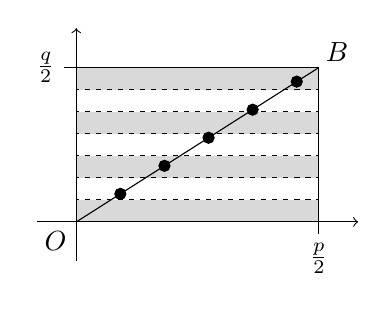
\begin{tikzpicture}[x=0.28cm,y=0.28cm]
				\foreach \ycoord in {0,2,4,6} \fill[black!15!white] (0,\ycoord) to (11,\ycoord) to (11,\ycoord+1) to (0,\ycoord+1) to cycle;
				\draw[->] (-0.5cm,0) to (11,0) to ++(0.5cm,0);
				\draw[->] (0,-0.5cm) to (0,7) to ++(0,0.5cm);
				\draw (11,-1ex) node[below] {$\frac p2$} to (11,7) to (-1ex,7) node[left] {$\frac q2$};
				\node[below left] at (0,0) {$O$};
				\node[shift={(40:2ex)}] at (11,7) {$B$};
				\foreach \ycoord in {1,2,3,4,5,6} \draw[line width=0.3,dash pattern=on 0.07cm off 0.07cm,dash phase=0.035cm] (0,\ycoord) to (11,\ycoord);
				\draw (0,0) to (11,7);
				\draw[fill=black] (2,2*7/11) circle (2pt);
				\draw[fill=black] (4,4*7/11) circle (2pt);
				\draw[fill=black] (6,6*7/11) circle (2pt);
				\draw[fill=black] (8,8*7/11) circle (2pt);
				\draw[fill=black] (10,10*7/11) circle (2pt);
			\end{tikzpicture} & & 
			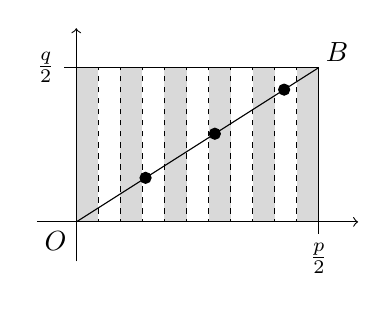
\begin{tikzpicture}[x=0.28cm,y=0.28cm]
				\foreach \xcoord in {0,2,4,6,8,10} \fill[black!15!white] (\xcoord,0) to (\xcoord+1,0) to (\xcoord+1,7) to (\xcoord,7) to cycle;
				\draw[->] (-0.5cm,0) to (11,0) to ++(0.5cm,0);
				\draw[->] (0,-0.5cm) to (0,7) to ++(0,0.5cm);
				\draw (11,-1ex) node[below] {$\frac p2$} to (11,7) to (-1ex,7) node[left] {$\frac q2$};
				\node[below left] at (0,0) {$O$};
				\node[shift={(40:2ex)}] at (11,7) {$B$};
				\foreach \xcoord in {1,2,...,10} \draw[line width=0.3,dash pattern=on 0.07cm off 0.07cm,dash phase=0.035cm] (\xcoord,0) to (\xcoord,7);
				\draw (0,0) to (11,7);
				\draw[fill=black] (2*11/7,2) circle (2pt);
				\draw[fill=black] (4*11/7,4) circle (2pt);
				\draw[fill=black] (6*11/7,6) circle (2pt);
			\end{tikzpicture} & & 
			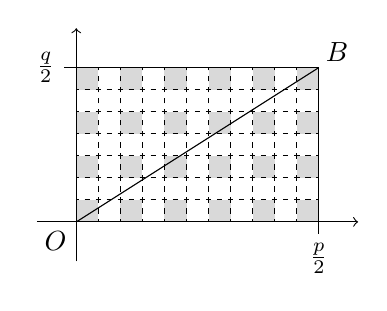
\begin{tikzpicture}[x=0.28cm,y=0.28cm]
				\foreach \xcoord in {0,2,4,6,8,10} {
					\foreach \ycoord in {0,2,4,6} \fill[black!15!white] (\xcoord,\ycoord) to (\xcoord+1,\ycoord) to (\xcoord+1,\ycoord+1) to (\xcoord,\ycoord+1) to cycle;
				}
				\draw[->] (-0.5cm,0) to (11,0) to ++(0.5cm,0);
				\draw[->] (0,-0.5cm) to (0,7) to ++(0,0.5cm);
				\draw (11,-1ex) node[below] {$\frac p2$} to (11,7) to (-1ex,7) node[left] 	{$\frac q2$};
				\foreach \xcoord in {1,2,...,10} \draw[line width=0.3,dash pattern=on 0.07cm off 0.07cm,dash phase=0.035cm] (\xcoord,0) to (\xcoord,7);
				\foreach \ycoord in {1,2,3,4,5,6} \draw[line width=0.3,dash pattern=on 0.07cm off 0.07cm,dash phase=0.035cm] (0,\ycoord) to (11,\ycoord);
				\node[below left] at (0,0) {$O$};
				\node[shift={(40:2ex)}] at (11,7) {$B$};
				\draw (0,0) to (11,7);
			\end{tikzpicture} & %\\
			%& horizontale Streifen & & vertikale Streifen  & & kleine Quadrate & 
		\end{tabularx}
	\end{figure}
	Analog können wir für $x=0,1,2,\dotsc,\frac{p-1}{2}$ den vertikalen Streifen aller Punkte $(s,t)$ betrachten, für die $x\leqslant s\leqslant x+\frac 12$ gilt. In der zweiten Abbildung sind diese vertikalen Streifen grau eingefärbt. Dann zählt $\frac{q-1}{2}-\nu$ wieviele der Punkte $\parens[\big]{\frac pqy,y}$ für $y=1,2,\dotsc,\frac{q-1}{2}$ in einem vertikalen grauen Streifen liegen. Die Überschneidungen der horizontalen und vertikalen grauen Streifen sind kleine Quadrate, die wir in der dritten Abbildung grau eingefärbt haben.
	
	Für jedes $x$ liegt der Punkt $\parens[\big]{x,\frac qpx}$ auf dem linken Rand eines vertikalen grauen Streifens. Also zählt $\frac{p-1}{2}-\mu$ auch, wie oft die Diagonale $\overline{OB}$ den linken Rand eines kleinen grauen Quadrats trifft. Analog zählt $\frac{q-1}{2}-\nu$ auch, wie oft die Diagonale $\overline{OB}$ den unteren Rand eines kleinen grauen Quadrates trifft (das kleine graue Quadrat mit Eckpunkt $O$ wird in beiden Fällen nicht mitgezählt). Folglich zählt
	\begin{equation*}
		\lambda\coloneqq\frac{p-1}{2}-\mu+\frac{q-1}{2}-\nu+1=\frac{p+q}{2}-(\mu+\nu)\,,
	\end{equation*}
	wieviele der kleinen grauen Quadrate die Diagonale $\overline{OB}$ schneidet (das $+1$ am Ende sorgt dafür, dass diesmal das Quadrat mit Eckpunkt $O$ mitgezählt wird). Da wir nur an der Parität von $\mu+\nu$ interessiert sind, müssen wir nur die Parität von $\lambda$ bestimmen, also die Parität der Anzahl der Schnitte von $\overline{OB}$ mit den kleinen grauen Quadraten.
	
	Wenn wir das Rechteck $OABC$ um seinen Mittelpunkt um $180^\circ$ drehen, wird $\overline{OB}$ auf sich selbst und jedes kleine graue Quadrat auf ein kleines graues Quadrat abgebildet. Damit können wir die kleinen grauen Quadrate, die von $\overline{OB}$ geschnitten werden, in Paare aufteilen -- es sei denn, eines der kleinen grauen Quadrate wird bei der Drehung auf sich selbst abgebildet. Dieses Quadrat müsste dann genau in der Mitte von $OABC$ sitzen. Ein solches Quadrat existiert genau dann, wenn die Anzahl der kleinen grauen Quadrate, also $\frac{p+1}{2}\cdot \frac{q+1}{2}$, ungerade ist. Wir sehen also, dass~$\lambda$ die gleiche Parität wie $\frac{p+1}{2}\cdot \frac{q+1}{2}$ hat. Folglich hat $-(\mu+\nu)=\lambda-\frac{p+q}{2}$ die gleiche Parität wie $\frac{p+1}{2}\cdot \frac{q+1}{2}-\frac{p+q}{2}=\frac{p-1}{2}\cdot \frac{q-1}{2}$. Also hat auch $\mu+\nu$ die gleiche Parität wie $\frac{p-1}{2}\cdot \frac{q-1}{2}$ und wir sind fertig!
\end{proof}

\subsection*{Beispielaufgaben}

Die Theorie der quadratischen Reste lässt sich auf vielfältige Weise in Olympiade-Aufgaben anwenden. Eine Anwendung haben wir im letzten Kapitel schon gesehen: Wir können sehr leicht bestimmen, ob eine gegebene Restklasse ein quadratischer Rest ist. Aber es gibt noch viele weitere Tricks, die ihr euch in den folgenden Aufgaben selbst erarbeiten sollt.

Wie üblich findet ihr am Ende des Kapitels Tricks zu den Aufgaben und am Ende des Heftes könnt ihr die Lösungen nachlesen.

%Wir beginnen mit einem weiteren Spezialfall des Primzahlsatzes von Dirichlet, den wir euch in \emph{Kapitel~\ref{kapitel:Ordnung}: Multiplikative Ordnungen und Primitivwurzeln} versprochen haben.
\begin{aufgabe*}\leavevmode\label{aufgabe:PrimzahlsatzVonDirichletMod4}
	\begin{enumerate}[label={$(\alph*)$},ref={$(\alph*)$}]
		\item Zeige, dass es unendlich viele Primzahlen $p$ mit $p\equiv 3\mod 4$ gibt.\label{teilaufgabe:3Mod4}
		\item Zeige, dass es unendlich viele Primzahlen $p$ mit $p\equiv 1\mod 4$ gibt.\label{teilaufgabe:1Mod4}
	\end{enumerate}
\end{aufgabe*}
\begin{aufgabe*}[*]\label{aufgabe:IMO1996_4}
	Seien $a$ und $b$ zwei positive ganze Zahlen mit der Eigenschaft, dass sowohl $15a+16b$ als auch $16a-15b$ Quadratzahlen sind. Finde den kleinstmöglichen positiven Wert, den das Minimum der beiden Quadratzahlen annehmen kann.
\end{aufgabe*}
\begin{aufgabe*}[*]\label{aufgabe:PrimfaktorTrick}
	Sei $a$ eine ganze Zahl. Zeige, dass die Zahlen $a^2+3$ und $a^2+5$ niemals Kubikzahlen sein können.
\end{aufgabe*}
Aufgabe~\ref{aufgabe:PrimfaktorTrick} benutzt einen Trick, der sehr gut zu wissen, aber nur sehr schwer zu finden ist. Benutzt also gerne die Tipps, dazu sind sie schließlich da.
\begin{aufgabe*}[**]\label{aufgabe:Polen2019}
	Sei~$p$ eine Primzahl und~$r$ eine Restklasse modulo~$p$, die $r^7\equiv 1\mod p$ erfüllt. Zeige: Wenn $r+1$ und $r^2+1$ quadratische Reste modulo~$p$ sind, dann ist auch $r^3+1$ ein quadratischer Rest modulo~$p$.
\end{aufgabe*}

\newpage\phantom{newpage}\vfill\hrule\vspace{-1em}
\subsection*{Tipps zu den Beispielaufgaben}

\textbf{Tipps zu Aufgabe~\ref{aufgabe:PrimzahlsatzVonDirichletMod4}.} Beide Teilaufgaben funktionieren ähnlich wie der übliche Beweis, dass unendlich viele Primzahlen existieren. Für~\ref{teilaufgabe:3Mod4} überlege dir, wie du erzwingen kannst, dass eine ganze Zahl einen Primfaktor $\equiv 3\mod 4$ besitzt. Für~\ref{teilaufgabe:1Mod4}, benutze den ersten Ergänzungssatz zum QRG.



\textbf{Tipps zu Aufgabe~\ref{aufgabe:IMO1996_4}.} Löse das lineare Gleichungssystem $15a+16b=m^2$, $16a-15b=n^2$. Welche Bedingungen müssen $m^2$ und $n^2$ erfüllen, damit die Lösungen ganzzahlig sind?

Zeige, dass $15$ kein quadratischer Rest modulo den Primfaktoren von $15^2+16^2$ ist.

\textbf{Tipps zu Aufgabe~\ref{aufgabe:PrimfaktorTrick}.} Um zu zeigen, dass $a^2+5=b^3$ keine Lösungen hat, schreibe die Gleichung in der Form $a^2+4=b^3-1$. Also muss $-4$ ein quadratischer Rest modulo jedem Primfaktor von $b^3-1$ sein. Folgere daraus einen Widerspruch.

Zu zeigen, dass $a^2+3=b^3$ keine Lösung hat, geht mit einem ähnlichen Argument (dieses braucht allerdings ein paar Schritte mehr).

\textbf{Tipps zu Aufgabe~\ref{aufgabe:Polen2019}.} Betrachte das Produkt $(r+1)(r^2+1)(r^3+1)$.

Wie lässt sich die Bedingung $r^7\equiv 1\mod p$ mithilfe einer Primitivwurzel modulo~$p$ ausdrücken? Zeige, dass~$r$ ein quadratischer Rest modulo~$p$ sein muss.
